\begin{figure}[H]
  \centering

  \begin{subfigure}[b]{0.2\textwidth}
    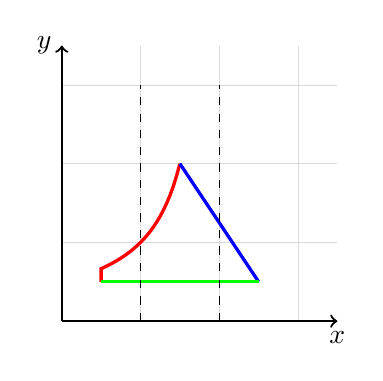
\begin{tikzpicture}

      \draw[very thin, gray!30, step = 1cm] (0, 0) grid (3.5, 3.5);
      \draw[color = red, very thick, domain = 0.5 : 1.5, variable = \x]
        (0.5, 0.5)
        -- plot ({\x}, {-1 / (\x - 2)});
      \draw[color = blue, very thick, domain = 1.5 : 2.5, variable = \x]
        (1.5, 2)
        -- plot ({\x}, {-1.5 * \x + 4.25});
      \draw[color = green, very thick] (0.5, 0.5) -- (2.5, 0.5);
    
      \draw[thick] [->] (0, 0) -- (3.5, 0) node[right, below] {\(x\)};
      \draw[thick] [->] (0, 0) -- (0, 3.5) node[above, left] {\(y\)};
      \draw[dashed] (1, 0) -- (1, 3);
      \draw[dashed] (2, 0) -- (2, 3);

    \end{tikzpicture}
  \caption{Неправильная в направлении \(Oy\) область}\label{fig:area-prop-2-a}
  \end{subfigure}
  \qquad
  \begin{subfigure}[b]{0.2\textwidth}
    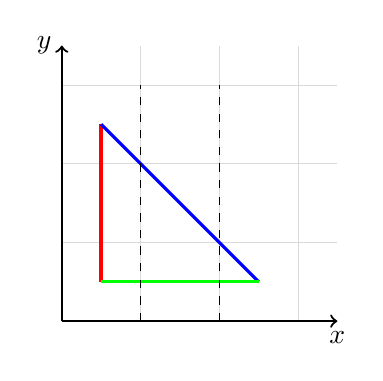
\begin{tikzpicture}

      \draw[very thin, gray!30, step = 1cm] (0, 0) grid (3.5, 3.5);
      \draw[color = red, very thick] (0.5, 0.5) -- (0.5, 2.5);
      \draw[color = blue, very thick] (0.5, 2.5) -- (2.5, 0.5);
      \draw[color = green, very thick] (0.5, 0.5) -- (2.5, 0.5);
    
      \draw[thick] [->] (0, 0) -- (3.5, 0) node[right, below] {\(x\)};
      \draw[thick] [->] (0, 0) -- (0, 3.5) node[above, left] {\(y\)};
      \draw[dashed] (1, 0) -- (1, 3);
      \draw[dashed] (2, 0) -- (2, 3);

    \end{tikzpicture}
    \caption{Правильная в направлении \(Oy\) область}\label{fig:area-prop-2-b}
  \end{subfigure}
\end{figure}